\section {Implementation and Technical Notes}

The code was run on a \textit{GTX 1080 Ti} and not the cluster of \textit{K'40s}. This could be a reason for variance in the optimal configuration found for the GPUs. However, the code does not make any hardware assumptions and can therefore be run on any suitable cluster. \\

CUDA version 9.0 was used to compile the code, with \lstinline{nvcc} as the device compiler and \lstinline{gcc} as the host compiler.

\section{Analysis of Problem Statement}

We are required to build N-count-grams of a given text (development on Shakespeare's \textit{Procreation Sonnets} ; test elsewhere). This is associated with a \textit{MAXWORD} limit. \\

Note that, unlike usual, we treat the whole text as a single sentence. 

\section{Pseudo Code}

\begin{enumerate}
\item  Read file, check if string is a word.
\item  Save words into an array.
\item For a given N, generate the sliding window array, with count. \textit{(Can this be optimised?)}
\item  Bin this histogram. \textit{(This can be optimised)}
\end{enumerate}

We shall implement ideas from shared memory atomics, privatisation etc, and also consider recent paper developments for this. Wherever this has helped, we shall cite the relevant papers for credibility.

\section{Implementing Binning}

We largely follow the following method:

\begin{itemize}
\item Declare shared memory with private output histogram
\item Cooperatively initialize the histogram to 0
\item Synchronize
\item Identify the index/indices of the input on which to operate. For each 
\begin{itemize}
\item Access each input item such that warps have coalesced access.
\item Use atomic add to update appropriate bin in the output histogram
\end{itemize}
\item Cooperatively update the global output histogram with local one with
\item atomic add
\end{itemize}

Now when N>5, we notice that shared memory can no longer fit our histograms, so we split the private histograms into private sub-histograms:

\begin{itemize}
\item Declare shared memory with private sub-histogram
\item Cooperatively initialize the histogram to 0
\item Synchronize
\item Identify the index/indices of the input on which to operate. For each 
\begin{itemize}
\item Ensure the global index you want to update falls in this sub-histogram.
\item Access each input item such that warps have coalesced access.
\item Use atomic add to update appropriate bin in the output histogram
\end{itemize}
\item Cooperatively update the global output histogram with local one with
\item atomic add
\end{itemize}

\section {Code and Timings}

Histogram binning via thread-wise access to shared memory was used. \\

We implement two kernels: one for the case of $N <5$ and one for the other (case of full privat. The results may be replicate histograms and the case of parallel ed by running,

\begin{lstlisting}[numbers = none]
./ee16b068.cu
\end{lstlisting}

\subsection{Run Timing and Interpretation}

\textbf{Figure-1} summarises the run-times (GPU kernel) for various \textit{N}, tested on the provided Shakespearean text.

\begin{figure}[ht]
\centering
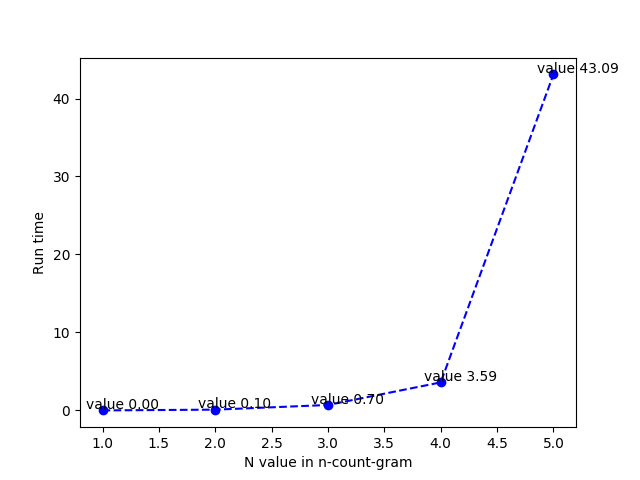
\includegraphics[angle=0,width=0.8\textwidth]{q1.png}
\caption{N-count-gram runtimes on\textbf{GTX1080 Ti}}
\end{figure}

This can be attributed to the fact that shared atomic collisions grow as the number of simultaneous additions increase, but a $log(n)$ dependency may be attributed to increased loops in each block. \\

For questions 2,3 , we shall consider column major timing only. \\

\subsection {Code Blocks for pre-processing, word-counts (pertinent only)}
\begin{lstlisting}
int checkWord(char* word,char* words,int* count_array,int offset){
    // Check if word meets, else pre-process
    // Args:
    // word >> word of consideration from fscanf
    // words >> Array where, every 20 chars is a word
    // offset >> Which entry to start writting at (modulo 20)
    // Returns:
    // new offset
    // Modifies:
    // words
    int loop=0;
    int count=0;

    for (loop=0;loop<strlen(word)-1;loop++)
    {
       
       if (word[loop]=='-')
       {
          words[offset*20+loop]=0;
          printf("Word %s \n",&words[offset*20]);
          offset+=1;
          count_array[offset]=count;
          count=0;
        }
       else{
          /* Copy character */
          words[offset*20+loop]=word[loop];
          count+=1;
       }
    }

    if (ispunct((unsigned char)word[strlen(word)-1]))
       {
          /* Skip this character */
          words[offset*20+strlen(word)-1]=0;
          count_array[offset]=count;
          offset+=1;
       }
    else{
        words[offset*20+strlen(word)-1]=word[strlen(word)-1];
        count+=1;
        words[offset*20+strlen(word)]=0;
        count_array[offset]=count;
        offset+=1;
    }
    return offset;

}

\end{lstlisting}
\bigskip

\subsection {Code Blocks for N=1,2,3,4 (pertinent only)}
\begin{lstlisting}
__global__ void nCountGram(int* d_count, int* d_hist, int N, int totalWordCount){
    extern __shared__ int buffer[];
    int *temp = &buffer[0];

    //__shared__ int temp[1024];
    // Helper var
    int index, j, p;
    int a, b;

    a=1;
    for (p=0;p<N;p++){
        a*=20;
    }

    for (p=0; p<a/1024+1; p++){
        if (threadIdx.x + p*1024< a){
            temp[threadIdx.x + p*1024] = 0;
        }
    }

    __syncthreads();

    int i = threadIdx.x + blockIdx.x * blockDim.x;
    int offset = blockDim.x * gridDim.x;

    while (i < totalWordCount - N + 1)
    {
        // Since 0,0 is invalid
        index=-1;
        b=a/20;
        for (j = 0;j < N; j++){
            index+=(d_count[i+j])*b;
            b/=20;
        }
        atomicAdd( &temp[index], 1);
        i += offset;
        //printf("Index %d",index);
    }

    __syncthreads();

    for (p=0;p<a/1024+1;p++){
        if (threadIdx.x + p*1024< a){
            atomicAdd( &(d_hist[threadIdx.x + p*1024]), temp[threadIdx.x + p*1024] );
            if (temp[threadIdx.x+p*1024]>0){
                //printf("Hist val at %d is %d \n",threadIdx.x+p*1024,d_hist[threadIdx.x + p*1024]);
            }
        }
    }

    __syncthreads();

}

\end{lstlisting}
\bigskip

\subsection {Code Blocks for N>=5 (pertinent only)}
\begin{lstlisting}
__global__ void nCountGram_optimal(int* d_count, int* d_hist, int N, int totalWordCount, int sub_hist_size){
    extern __shared__ int buffer[];
    int *temp = &buffer[0];

    //__shared__ int temp[1024];
    // Helper var
    int index, j, p;
    int a, b;

    a=1;
    for (p=0;p<N;p++){
        a*=20;
    }

    for (p=0; p<sub_hist_size/1024 +1; p++){
        if (threadIdx.x + p*1024 < sub_hist_size){
            temp[threadIdx.x + p*1024] = 0;
        }
    }

    __syncthreads();

    int i = threadIdx.x + blockIdx.x * blockDim.x ;//blockIdx.y*gridDim.y;
    int offset = blockDim.x * gridDim.x*blockIdx.y*gridDim.y;

    while (i < totalWordCount - N + 1)
    {
        // Since 0,0 is invalid
        index=-1;
        b=a/20;
        for (j = 0;j < N; j++){
            index+=(d_count[i+j])*b;
            b/=20;
        }
        if ((index<sub_hist_size*(blockIdx.y+1)) && (index > sub_hist_size*blockIdx.y)){
            //printf("Index %d",index);
        atomicAdd( &temp[index - blockIdx.y*sub_hist_size], 1);
        }
        i += offset;
    }

    __syncthreads();

    for (p=0;p<sub_hist_size/1024+1;p++){
        if (threadIdx.x + p*1024 < sub_hist_size){
            atomicAdd( &(d_hist[threadIdx.x + sub_hist_size*blockIdx.y + p*1024]), temp[threadIdx.x + p*1024] );
            if (d_hist[threadIdx.x+ sub_hist_size*blockIdx.y + p*1024]>0){
                printf("Hist val at %d is %d \n",threadIdx.x+sub_hist_size*blockIdx.y+p*1024,d_hist[threadIdx.x +sub_hist_size*blockIdx.y+ p*1024]);
            }
        }
    }

    __syncthreads();

}

\end{lstlisting}
\bigskip

\section{References}
\begin{itemize}
\item Classroom lectures and Slides.
\item CUDA Dev Documentation.
\end{itemize}

